\documentclass[../Article_Model_Parameters.tex]{subfiles}
\graphicspath{{\subfix{../Figures/}}}
\begin{document}
	
	\label{CH: Gouverning equations}
	
	\subsubsection{Mass continuity}

	Following the work of \citet{Anderson1995}, the governing equations for compressible fluid with non-uniform cross-section can be obtained. Let's assume that any properties of the flow are uniform across any given cross-section of an extractor. The variation of the cross-section might result from the partial filling of an extractor or its irregular shape. In reality, such a flow is two-dimensional because the area changes as a function of $z$, and there is a flow-field variation in both directions. The assumption of quasi-one-dimensional flow dictates that the flow properties are a function of $z$ only. The integral form of the continuity equation is:
	
	{\footnotesize
		\begin{equation}
			\cfrac{\partial}{\partial t} \iiint_{\mathcal{V}_f} \rho_f d\mathcal{V}_f + \iint_S \rho_f \textbf{V} \cdot \textbf{dS} = 0
			\label{EQ: Continuity_integral_general}
		\end{equation}
	}
	
	We apply this equation to the shaded control volume shown in Figure \ref{fig: control_volume}. 
	
	\begin{figure}[h]
		\centering
		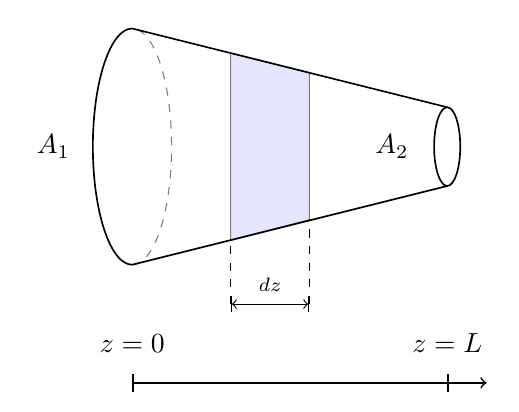
\begin{tikzpicture}
			\draw [fill=blue!20!white,opacity=0.5] (2.25,2.44) -- (2.25,0.57) -- (1.25,0.31) -- (1.25,2.69) -- cycle;%smmall triangle
			\draw[dashed,color=gray] (0,0) arc (-90:90:0.5 and 1.5);% right half of the left ellipse
			\draw[semithick] (0,0) -- (4,1);% bottom line
			\draw[semithick] (0,3) -- (4,2);% top line
			\draw[semithick] (0,0) arc (270:90:0.5 and 1.5);% left half of the left ellipse
			\draw[semithick] (4,1.5) ellipse (0.166 and 0.5);% right ellipse
			\draw (-1,1.5) node {$A_1$};
			\draw (3.3,1.5) node {$A_2$};
			\draw[|-,semithick] (0,-1.5) -- (4,-1.5);
			\draw[|->,semithick] (4,-1.5) -- (4.5,-1.5);
			\draw (0,-1) node {$z=0$};
			\draw (4,-1) node {$z=L$};
			\draw (1.75,-0.25) node{\scriptsize $ dz $}; %a number
			\draw[|<->|] (1.25,-0.5) -- (2.25,-0.5); %lenght indicator
			\draw[dashed] (1.25,-0.5) -- (1.25,0.3); %dashed line
			\draw[dashed] (2.25,-0.5) -- (2.25,0.58); %dashed line
		\end{tikzpicture}
		\caption{Control volume for deriving the partial differential equation for unsteady, quasi-one-dimensional flow}
		\label{fig: control_volume}
	\end{figure}
	
	 On the left side of the control volume, consistent with the quasi-one-dimensional assumptions, the density, velocity, pressure, and internal energy denoted by $\rho_f$, $v$, $P$, and $e$, respectively, are uniform over the area $A$. Similarly, on the right side of the control volume, the density, velocity, pressure, and internal energy $\rho_f+d\rho_f$, $v+dv$, $P+dP$, and $e+de$, respectively, are uniform over the area available for fluid phase $A_f+dA_f$. Applied to the control volume in Figure \ref{fig: control_volume}, the volume integral in Equation \ref{EQ: Continuity_integral_general} becomes, in the limit as $dz$ becomes very small,
	
	{\footnotesize
		\begin{equation}
			\cfrac{\partial}{\partial t} \iiint_{\mathcal{V}_f} \rho_f d\mathcal{V}_f = \cfrac{\partial}{\partial t}\left( \rho_f A_f dz \right)
			\label{EQ: Cont_Simpl_Vol}
		\end{equation}
	}

	where $A~dz$ is the volume of the control volume in the limit of $dz$ becoming vanishingly small. The surface integral in Equation \ref{EQ: Continuity_integral_general} becomes
	
	{\footnotesize
		\begin{equation}
			\iint_S \rho_f \textbf{V} \cdot \textbf{dS} = -\rho_f v A_f + (\rho_f+d\rho_f)(v+dv)(A_f+dA_f)
		\end{equation}
	}

	The minus sign on the leading term on the right-hand side is due to the vectors $\textbf{V}$ and $\textbf{dS}$ pointing in opposite directions over the left of the control volume, and hence the dot product is negative. Expanding the triple product term 
	 
	{\footnotesize
		\begin{align}
			&\iint_S \rho_f \textbf{V} \cdot \textbf{dS} = -\rho_f v A_f + \rho_f v A_f + \rho_f v dA_f + \rho_f A_f dv \nonumber \\ 
			&+ \rho_f dv dA_f + v A_f d\rho_f + v d\rho_f dA + A_f d\rho_f dv + d\rho_f dv dA_f
			\label{EQ: Triple_Prod_Cont_Surf}
		\end{align}
	}
	
	In the limit as $dz$ becomes very small, the terms involving products of the differential in Equation \ref{EQ: Triple_Prod_Cont_Surf}, such as $\rho_f dv dA_f,~d\rho_f dv dA_f$, go to zero much faster than those terms involving only one differential. Hence, all terms involving products of differentials can be dropped, yielding in the limit as $dz$ becomes very small
	
	{\footnotesize
		\begin{equation}
			\iint_S \rho_f \textbf{V} \cdot \textbf{dS} = \rho_f v dA_f + \rho_f A_f dv + v A_f d\rho_f 
			\label{EQ: Cont_Simpl_Surf}
		\end{equation}
	}

	Substituting Eqs. \ref{EQ: Cont_Simpl_Vol} and \ref{EQ: Cont_Simpl_Surf} into \ref{EQ: Continuity_integral_general}, we have
	
	{\footnotesize
		\begin{equation}
			\cfrac{\partial \left( \rho_f A_f \right)}{\partial t} + \cfrac{\partial \left( \rho_f A_f v \right)}{\partial z} = 0
			\label{EQ: Conservative_continuity}
		\end{equation}
	}
	
	The above partial differential equation form of the continuity equation is suitable for unsteady, quasi-one-dimensional flow. The $A_f(z)$ is an arbitrary function that describes a change in the extractor's cross-section and can be defined as $A_f(z) = \textbf{A} \phi(z)$, where $\phi$ is the bed porosity and $\textbf{A}$ is the cross-section of an empty extractor.
	
	{\footnotesize
		\begin{equation}
			\cfrac{\partial \left( \rho_f \textbf{A} \phi (z) \right)}{\partial t} + \cfrac{\partial \left( \rho_f \textbf{A} \phi (z) v \right)}{\partial z} = 0
		\end{equation}
	}
	The equation can be simplified by canceling out $\textbf{A}$
	
	{\footnotesize
		\begin{equation}
			\cfrac{\partial \left( \rho_f \phi (z) \right)}{\partial t} + \cfrac{\partial \left( \rho_f \phi (z) v \right)}{\partial z} = 0
		\end{equation}
	}
	
	If so-called superficial velocity is defined as $u=\phi v$, the mass continuity becomes
	
	{\footnotesize
		\begin{equation}
			\cfrac{\partial \left( \rho_f \phi (z) \right)}{\partial t} + \cfrac{\partial \left( \rho_f u \right)}{\partial z} = 0
			\label{EQ: Mass_Continuity}
		\end{equation}
	}
	
	\subsubsection{Transport of a species}
	
	The transport of a solute, can be described by an analogous equation to the Equation \ref{EQ: Continuity_integral_general} with additional terms on the right-hand side. The first term on the right-hand side describes diffusional movement of species and is based on the Fick's law $\left( J_{diff} = D_e^M\frac{\partial c_f}{\partial z} \right)$. The other term corresponds to the mass transfer between solid and fluid phases, which is treated as a source term.
	
	{\footnotesize
		\begin{equation}
			\cfrac{\partial}{\partial t} \iiint_{\mathcal{V}_f} c_f d\mathcal{V}_f + \iint_S c_f \textbf{V} \cdot \textbf{dS} = \iint_S J_{diff} \cdot \textbf{n}~\textbf{dS} + \cfrac{\partial}{\partial t} \iiint_{\mathcal{V}_s} c_s d\mathcal{V}_s
			\label{EQ: Integral_Mass_Species_general}
		\end{equation}
	}
	
	Similarly to the continuity equation, in the limit as $dz$ becomes very small
	
	{\footnotesize
		\begin{align}
			\cfrac{\partial}{\partial t} \iiint_{\mathcal{V}_f} c_f d\mathcal{V}_f &= \cfrac{\partial}{\partial t}\left( c_f A_f dz \right) \\
			\cfrac{\partial}{\partial t} \iiint_{\mathcal{V}_s} c_s d\mathcal{V}_s &= \cfrac{\partial}{\partial t}\left( c_s A_s dz \right)
		\end{align}
	}

	The surface integrals in the limit of $dz$ become
	
	{\footnotesize
		\begin{equation}
			\iint_S c_f \textbf{V} \cdot \textbf{dS} = c_f v dA_f + c_f A_f dv + v A_f dc_f 
		\end{equation}
	}
	
	From the Divergence theorem in multi-variable calculus, we have
	
	{\footnotesize
		\begin{equation}
			\iint_S J_{diff} \cdot \textbf{n}~\textbf{dS} = \iiint_{\mathcal{V}_f} \nabla J_{diff} dv_f = \nabla \iiint_{\mathcal{V}_f} J_{diff} dv_f = \nabla \left( J_{diff} A_f dz \right)
		\end{equation}
	}
	
	By substituting the equations derived above into Equation \ref{EQ: Integral_Mass_Species_general} we obtain
	
	{\footnotesize
		\begin{equation}
			\cfrac{\partial \left( c_f A_f \right)}{\partial t} + \cfrac{\partial \left( c_f A_f v \right)}{\partial z} = \cfrac{\partial \left( c_s A_s \right) }{\partial t} + \cfrac{\partial \left( J_{diff} A_f \right) }{\partial z}
		\end{equation}
	}

	By defining $A_f = A \cdot \phi$, $A_s = A \cdot \left( 1-\phi \right)$ and $u=V \cdot \phi$, and assuming that $A$ is constant, the above equation becomes
	
	{\footnotesize
		\begin{equation}
			\cfrac{\partial \left( c_f \phi \right)}{\partial t} + \cfrac{\partial \left( c_f u\right)}{\partial z} = \cfrac{\partial \left( c_s (1-\phi) \right) }{\partial t} + \cfrac{\partial \left( J_{diff} \phi \right) }{\partial z}
		\end{equation}
	}

	By assuming that ${\footnotesize \frac{\partial \phi}{\partial t}=0}$ and expanding $J_{diff}$, we get
	
	{\footnotesize
		\begin{equation}
			\cfrac{\partial c_f}{\partial t} + \cfrac{1}{\phi} \cfrac{\partial \left( c_f u\right)}{\partial z} = \cfrac{ (1-\phi)}{\phi} \cfrac{\partial c_s }{\partial t} + \cfrac{1}{\phi} \cfrac{\partial}{\partial z} \left( D_e^M \cfrac{\partial c_f}{\partial z} \right)
		\end{equation}
	}
	
	The equation can be further simplified if $\frac{\partial u}{\partial z} = \frac{\partial \phi}{\partial z} = D_e^M = 0$, which corresponds to the assumptions of constant velocity along the bed( which might be a case of isothermal and low-Mach number flow), constant porosity( which comes from the assumption of constant area for both solid and fluid phase) and no radial diffusion.
	
	{\footnotesize
		\begin{equation}
			\cfrac{\partial c_f}{\partial t} + \cfrac{u}{\phi} \cfrac{\partial c_f}{\partial z}  = \cfrac{1-\phi}{\phi} \cfrac{\partial c_s}{\partial t} 
			\label{EQ: Simplified_Species_Conservation}
		\end{equation}
	}

	The Equation \ref{EQ: Simplified_Species_Conservation} is equivalent to the equation presented by \citet{Reverchon1996}.
	
	\begin{comment}
	\subsubsection{Momentum conservation}
	
	Similarly to mass conservation, momentum conservation is derived for inviscid fluid with no body forces
	
	{\footnotesize
		\begin{equation}
			\cfrac{\partial}{\partial t} \iiint_{\mathcal{V}_f} \left( \rho_f v_z \right) d\mathcal{V}_f + \iint_S \left( \rho_f v_z \textbf{V} \right) \textbf{dS} = \iint_S \left( P dS \right)_z
			\label{EQ: Momentum_Integral_Form}
		\end{equation}
	}
	where $V_z$ is the $z$ component of the velocity.

	We the momentum conservation to the shaded control volume in Figure \ref{fig: control_volume}, the integrals on the left side are evaluated in the same manner as discussed above in the regard to the continuity equation. That is,
	
	{\footnotesize
		\begin{equation}
			\cfrac{\partial}{\partial t} \iiint_{\mathcal{V}_f} \left( \rho_f v_z \right) d \mathcal{V}_f = \cfrac{\partial}{\partial t} \left( \rho_f v A_f dz \right)
			\label{EQ: Force_Continuity_Monenmtum}
		\end{equation}equation
	}
	
	and 
	
	{\footnotesize
		\begin{equation}
			\iint_S \left( \rho_f v_z \textbf{V} \right) dS = -\rho_f v^2 + \left( \rho_f + d \rho_f \right) \left( v+dv \right)^2 \left( A+dA \right)
		\end{equation}
	}
	
	\begin{figure}[h]
		\centering
		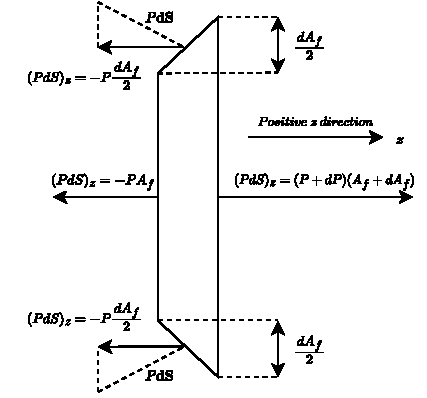
\includegraphics[width=\columnwidth]{Forces.pdf}
		\caption{The forces in the $z$ direction acting on the control volume}
		\label{fig: Forces_Momentum_Control_Volume}
	\end{figure}
	
	The evaluation of the pressure force term on the right side of Equation \ref{EQ: Momentum_Integral_Form} can be understood based on the Figure \ref{fig: Forces_Momentum_Control_Volume}. Here, the $z$ components of the vector $PdS$ are shown on all four sides of the control volume. Remember that $\textbf{dS}$ is assumed to point away from the control volume; hence  any $z$ component $\left( PdS \right)_z$ that acts toward the left (in the negative $z$ direction) is a negative quantity. Any $z$ component that acts toward the right (in the positive $z$ direction) is a positive quantity. Also note that the $z$ component of $P\textbf{dS}$ acting on the top and the bottom inclined faces of the control volume in Figure \ref{fig: Forces_Momentum_Control_Volume} can be expressed as the pressure $P$ acting on the component of the inclined is projected perpendicular to the $z$ direction, $dA_f/2$; hence, the contribution of each inclined face (top or bottom) to the pressure integral in Equation \ref{EQ: Momentum_Integral_Form} is $-P(dA_f/2)$. All together, the right-hand side of Equation \ref{EQ: Momentum_Integral_Form} is expressed as follows:
	
	{\footnotesize
		\begin{equation}
			\iint \left( PdS \right)_z = -PA_f + (P+dP)(A+dA_f)-2P\cfrac{dA_f}{2}
			\label{EQ: Force_Integral_Varying_Cross_Section}
		\end{equation}
	}
	
	Substituting Eqs. \ref{EQ: Force_Continuity_Monenmtum} to \ref{EQ: Force_Integral_Varying_Cross_Section} into Equation \ref{EQ: Momentum_Integral_Form}, we have
	
	{\footnotesize
		\begin{align}
			& \cfrac{\partial}{\partial t} \left( \rho_f v A_f dz \right) - \rho_f v^2 A_f + (\rho_f + d\rho_f)(v+dv)^2(A_f+dA_f)  \nonumber \\
			&= PA_f - (P+dP)(A+dA_f)+PdA_f
		\end{align}
	}
	
	Canceling like terms and ignoring products of differentials, the equation above becomes in the limit $dz$ becoming  very small
	
	{\footnotesize
		\begin{equation}
			\cfrac{\partial}{\partial t} \left( \rho_f v A_f dz \right) + d\left( \rho_f v^2 A_f \right) = -A dP
		\end{equation}
	}

	Dividing the above equation by $dz$ and taking the limit as $dz$ goes to zero, we obtain
	
	{\footnotesize
		\begin{equation}
			\cfrac{\partial \left( \rho_f v A_f \right)}{\partial t} + \cfrac{\partial \left( \rho_f v^2 A_f \right)}{\partial z} = -A_f \cfrac{\partial P}{\partial z}
			\label{EQ: Conservative_Momentum}
		\end{equation}
	}

	The Equation \ref{EQ: Conservative_Momentum} can be expanded further by assuming that $A_f = \textbf{A}\phi$ 
	
	{\footnotesize
		\begin{equation}
			\cfrac{\partial \left( \rho_f v \textbf{A} \phi \right) }{\partial t} + \cfrac{\partial \left( \rho_f v^2 \textbf{A} \phi \right) }{\partial z} = - 	\textbf{A} \phi \cfrac{\partial P}{\partial t}
		\end{equation}
	}

	The equation can be further simplified by assuming that the cross-section of an extractor $\textbf{A}$ is constant and cancel out
	
	{\footnotesize
		\begin{equation}
			\cfrac{\partial \left( \rho_f v \phi \right) }{\partial t} + \cfrac{\partial \left( \rho_f v^2 \phi \right) }{\partial z} = - \phi 	\cfrac{\partial P}{\partial t}
		\end{equation}
	}

	If the superficial velocity $u=\phi V$ is introduced, then the momentum conservation becomes
	
	{\footnotesize
		\begin{equation}
			\cfrac{\partial \left( \rho_f u \right)}{\partial z} + \cfrac{\partial \left( \rho_f u^2/\phi \right) }{\partial z} = -\phi \cfrac{\partial 	P}{\partial z}
		\end{equation}
	}

	Equation \ref{EQ: Conservative_Momentum} represents the conservative form of the momentum equation for the quasi-one-dimensional flow. The equivalent non-conservative form can be obtained by multiplying the continuity equation by $v$ and subtracting it from Equation \ref{EQ: Conservative_Momentum}
	
	{\footnotesize
		\begin{equation}
			\cfrac{\partial \left( \rho_f v A_f \right)}{\partial t} - V\cfrac{ \partial \left( \rho_f A_f \right) }{\partial t} + \cfrac{\left( \rho_f v^2 A_f 	\right)}{\partial z} - V \cfrac{\left( \rho_f v A_f \right)}{\partial z} = -A_f \cfrac{\partial P}{\partial z}
		\end{equation}
	}
	
	Expanding the derivatives on the left-hand side of the above equation and canceling like terms, gives

	{\footnotesize
		\begin{equation}
			\rho_f A_f \cfrac{\partial v}{\partial t} + \rho_f A_f v \cfrac{\partial v}{\partial z} = -A_f \cfrac{\partial P}{\partial z}
		\end{equation}
	}

	Dividing the above equation by $A_f$ the non-conservative form of the momentum can be obtained
	
	{\footnotesize
		\begin{equation}
			\rho_f \cfrac{\partial v}{\partial t} + \rho_f v \cfrac{\partial v}{\partial z} = -\cfrac{\partial P}{\partial z}
			\label{EQ: Non-conservative_Momentum}
		\end{equation}
	}

	The Equation \ref{EQ: Non-conservative_Momentum} is stylistically the same as the general momentum conservation for one-dimensional flow with no-body forces. The momentum equation can be expressed in terms of superficial velocity $u=v\phi$. 
	
	{\footnotesize
		\begin{equation}
			\rho_f \cfrac{\partial \left(u / \phi \right)}{\partial t} + \rho_f \cfrac{u}{\phi} \cfrac{\partial \left( u / \phi \right)}{\partial z} = - \cfrac{\partial P}{\partial z}
		\end{equation}
	}

	By expanding all the terms of the equation above, we get
	
	{\footnotesize
		\begin{equation}
			\cfrac{\rho_f}{\phi} \cfrac{\partial u}{\partial t} + \rho_f u \cfrac{\partial \phi^{-1}}{\partial t} + \rho_f \cfrac{u}{\phi} \cfrac{1}{\phi} \cfrac{\partial u}{\partial z} + \rho_f \cfrac{u}{\phi} u \cfrac{\partial \phi^{-1} }{\partial z} = - \cfrac{\partial P}{\partial z}
		\end{equation}
	}
	
	If the bed is not compressible and doesn't change its properties during the batch, then ${\footnotesize\cfrac{\partial \phi}{\partial t}=0}$
	
	{\footnotesize
		\begin{equation}
			\cfrac{\rho_f}{\phi} \left( \cfrac{\partial u}{\partial t} + \cfrac{u}{\phi} \cfrac{\partial u}{\partial z} + u^2 \cfrac{\partial \phi^{-1}}{\partial z} \right) = -\cfrac{\partial P}{\partial z}
		\end{equation}
	}

	If the porosity is constant along an extractor, then the momentum conservation equation becomes
	
	{\footnotesize
		\begin{equation}
			\cfrac{\rho_f}{\phi} \left( \cfrac{\partial u}{\partial t} + \cfrac{u}{\phi} \cfrac{\partial u}{\partial z} \right) = -\cfrac{\partial P}{\partial z}
			\label{EQ: Non-conservative_Momentum_Const_Porosity}
		\end{equation}
	}

	The Equation \ref{EQ: Non-conservative_Momentum_Const_Porosity} represents the non-conservative form of the momentum equation for quasi-one-dimensional flow with no body forces and constant porosity.
	
	\subsubsection{Energy conservation}
	
	Let's consider the integral form of the energy equation for adiabatic flow with no body forces and no viscous effects
	
	{\footnotesize
		\begin{equation}
			\cfrac{\partial}{\partial} \iiint_{\mathcal{V}_f} \rho_f \left( e_f + \cfrac{v^2}{2} \right) d\mathcal{V}_f + \iint_S \rho_f \left( e_f + \cfrac{v^2}{2} \right) \textbf{V} \cdot \textbf{dS} = - \iint_S \left( P\textbf{V} \right) \cdot \textbf{dS}
			\label{EQ: Energy_equation_integral}
		\end{equation}
	}

	Applied to the shaded control volume in Figure \ref{fig: control_volume}, and keeping in mind the pressure forces shown in Figure \ref{fig: Forces_Momentum_Control_Volume}, Equation \ref{EQ: Energy_equation_integral} becomes
	
	{\footnotesize
		\begin{align}
			&\cfrac{\partial}{\partial t} \left[ \rho_f \left( e_f + \cfrac{v^2}{2} \right) A_f dz \right] - \rho_f \left( e_f + \cfrac{v^2}{2} \right) v A_f \nonumber \\
			&+ \left( \rho_f + d\rho_f \right) \left[ e_f + de_f + \cfrac{\left( v + dv \right)^2}{2} \right] \left( V+dV \right) \left( A_f+dA_f \right) \nonumber \\
			&= - \left[ -PvA_f + \left(P+dP\right) \left(v+dv\right) \left(A_f+dA_f\right) - 2\left( Pv\cfrac{dA_f}{2} \right) \right]
		\end{align}
	} %\todo[]{Check fV}
	
	Neglecting products of differential and canceling like terms, the above equation becomes
	
	{\footnotesize
		\begin{equation}
			\cfrac{\partial}{\partial t} \left[ \rho_f \left( e_f + \cfrac{v^2}{2} \right) A_f dz \right] + d\left( \rho_f r_f A_f \right) + \cfrac{ \left( \rho_f v^3 A_f \right) }{2} = -d \left( P A_f v \right)
		\end{equation}
	}

	or
	
	{\footnotesize
		\begin{equation}
			\cfrac{\partial}{\partial t} \left[ \rho_f \left( e_f + \cfrac{v^2}{2} \right) A_f dz \right] + d \left[ \rho_f \left( e_f \cfrac{v^2}{2} \right) vA_f \right] = - d\left( P A_f v \right)
		\end{equation}
	}

	Taking the limit as $dz$ approaches zero, the equation above becomes the following partial differential equation
	
	{\footnotesize
		\begin{equation}
			\cfrac{\partial \left[ \rho_f \left( e_f + v^2 / 2 \right) A \right]}{\partial t} + \cfrac{\partial \rho_f \left( e_f + v^2 / 2 \right)vA_f}{\partial z} = -\cfrac{\partial \left( P A_f v \right)}{\partial z}
			\label{EQ: Energy_equation_conservative_total}
		\end{equation}
	}
	
	Equation \ref{EQ: Energy_equation_conservative_total} is the conservation form of the energy expressed in terms of the total energy $e~+~v^2/2$, appropriate for unsteady, quasi-one-dimensional flow. The energy equation can be expressed in terms of internal energy if Equation \ref{EQ: Conservative_Momentum} is multiplicated by $v$ and then subtracted from Equation \ref{EQ: Energy_equation_conservative_total}
	
	{\footnotesize
		\begin{equation}
			\cfrac{\partial \left( \rho_f e_f A_f \right) }{\partial t} + \cfrac{\partial \left( \rho_f  e_f v A_f \right)}{\partial z} = -P \cfrac{\partial A_f v}{\partial z}
			\label{EQ: Energy_conservative_internal}
		\end{equation}
	}
	
	The equation above is the conservation form of the energy equation expressed in terms of internal energy $e_f$ suitable for quasi-one-dimensional flow. The non-conservative for is then obtained by multiplying the continuity equation \ref{EQ: Conservative_continuity}, by $e_f$ and substructing it from \ref{EQ: Energy_conservative_internal}, yielding 
	
	{\footnotesize
		\begin{equation}
			\rho_f A_f \cfrac{\partial e_f}{\partial t} + \rho_f A_f v \cfrac{\partial e_f}{\partial z} = - P \cfrac{\partial (A_f v) }{\partial z}
		\end{equation}
	}
	
	Expanding the right-hand side and dividing by $A_f$, the above equation becomes 
	
	{\footnotesize
		\begin{equation}
			\rho_f \cfrac{\partial e_f}{\partial t} + \rho_f v \cfrac{\partial e_f}{\partial z} = -P \cfrac{v}{A_f} \cfrac{\partial A_f}{\partial z}
		\end{equation}
	}

	or
	
	{\footnotesize
		\begin{equation}
			\rho_f \cfrac{\partial e_f}{\partial t} + \rho_f v \cfrac{\partial e_f}{\partial z} = -P \cfrac{\partial v}{\partial z} - P V \cfrac{\partial (ln~A_f)}{\partial z}
			\label{EQ: Energy_equation_nonconservative}
		\end{equation}
	}
	
	Equation \ref{EQ: Energy_equation_nonconservative} is the non-conservative form of the energy equation expressed in terms of internal energy, appropriate to unsteady quasi-one-dimensional flow. The reason for obtaining the energy equation in the form of Equation \ref{EQ: Energy_equation_nonconservative} is that, for a calorically perfect gas, it leads directly to a form of the energy equation in terms of temperature $T$. 
%	
%	For calorically perfect gas ${\footnotesize e_f=C_vT}$
%	
%	\hrule
%	
%	{\footnotesize
%		\begin{equation}
%			\cfrac{\partial \left( \rho_f e_f A_f \right) }{\partial t} + \cfrac{\partial \left( \rho_f  e_f v A_f \right)}{\partial z} = -P \cfrac{\partial A_f v}{\partial z} + \cfrac{\partial}{\partial z} \left( k \cfrac{\partial T}{\partial z} \right)
%		\end{equation}
%	}
	
%	{TODO: \color{red}finish derivation of energy equation for real gas and introduce a homogenous version of the energy equation}
	
\end{comment}
	
	
	
	
	
	
	
	
	
	
	
	
\end{document}